%!TEX root = ComputerScienceOne.tex

%%Chapter: Arrays

Rarely do we ever deal with a single piece of data in a program.  Instead, 
most data is made up of a collection of similar elements.  A program to
compute grades would be designed to operate on an entire roster of 
students.  Scientific data represents a collection of many different samples.
A bank maintains and processes many different accounts, etc.

\emph{Arrays} are a way to collect similar pieces of data together in an
\emph{ordered collection}.  The pieces of data stored in an array are
referred to as \emph{elements} in an ordered manner.  That is, there is 
a ``first'' element, ``second'' element, etc. and a ``last'' element.  Though
the elements are ordered, they are not necessarily \emph{sorted} in any 
particular manner.  Instead, the order is usually determined by the order
in which you place elements into the array.

Some languages only allow you to store the same types of elements in
an array.  For example, an integer array would only be able to store integers, 
an array of floating-point numbers would only be able to store floating-point
numbers.  Other languages allow you to create arrays that can hold 
\emph{mixed elements}.  A mixed array would be able to hold elements
of any type, so it could hold integers, floating-point numbers, strings, objects, 
or even other arrays.

Some languages treat arrays as full-fledged object types that have 
not only elements as their content, but methods that can be called
to manipulate or transform the contents of the array.  Other languages
treat arrays as a more primitive type, simply using arrays as storage
data structures.

Languages can vary greatly in how they implement and represent
arrays of elements, but many have the same basic usage patterns
allowing you to create arrays and manipulate their contents.

\section{Basic Usage}

\subsubsection{Creating Arrays}

Though there can be great variation in how a language uses arrays,
there are some commonalities.  Languages may allow you to create
\emph{static} arrays or \emph{dynamically allocated arrays} (see
Section \ref{section:arraysInDepth} below for a detailed discussion).  Static
arrays are generally created using the program stack space while 
dynamically allocated arrays are stored in the \emph{heap}.  In either
case you generally declare an array by specifying its size.  In statically
typed languages, you must also declare the array's type (integer, 
floating-point, etc.).

\subsubsection{Indexing Arrays}

Once an array has been created you can use it by assigning values
to it or by retrieving values from it.  Because there is more than one
element, you must specify \emph{which} element you are assigning
or retrieving.  This is generally done through \emph{indexing}.  An 
\emph{index} is an integer that specifies an element in the array.
The index is used in conjunction with (usually) square brackets and
the array's identifier.  For example, if the array's identifier is 
\mintinline{c}{arr} and the index is an integer value stored in the 
variable \mintinline{c}{i}, we would refer to the $i$-th element using
the syntax \mintinline{c}{arr[i]}.

For most programming languages, indices start at zero.  This is 
known as zero-indexing.\footnote{Though, some languages do 
use 1-indexing, there are very strong arguments in favor of 
zero-indexing \cite{Dijkstra82}.} Thus, the first element is at 
\mintinline{c}{arr[0]}, the second at \mintinline{c}{arr[1]}
etc.  When an array is stored in memory, each element is usually 
stored one after the other in one contiguous space in memory.  
Further, each element is of a specific type which is represented
using a fixed number of bytes in memory.  Thus the index actually
acts as an \emph{offset} in memory from the beginning of the
array.  For example, if we have an array of integers which each take
4 bytes each, then the 5th element would be stored at index $4$, 
which is an an offset equal to $4 \times 4 = 16$ bytes away from the 
beginning of the array.  The first element, being at index $0$ is thus
at $4 \times 0 = 0$ bytes from the beginning of the array (that is, 
the first element is at the beginning of the array).

Once an element has been indexed, it can essentially be treated as
a regular variable, assigning and retrieving values as you would regular
variables.  Care must be taken so that you do not make a reference
to an element that does not exist.  For example, using a negative
index or an index $i \geq n$ in an array of $n$ elements.  Depending
on the language, index an array element that is out-of-bounds may
result in undefined behavior, an exception being thrown, or a
corruption of memory.

\subsubsection{Iteration}

Since we can simply index elements in an array, it is natural to
iterate over elements in an array using a for-loop.  We can create
a for-loop using an index variable $i$ which starts at 0, and increments
by one on each iteration, accessing the $i$-th element using the
syntax described above, \mintinline{c}{arr[i]}.  One issue is that
such a loop would need to know how large the array is in order
to define a terminating condition.  

\begin{algorithm}
$n \leftarrow$ size of array $arr$ \;
\For{$i=0, \ldots, (n-1)$}{
  process element $arr[i]$ \;
}
\end{algorithm}

Some languages build the size of the array into a property that 
can be accessed.  Java, for example, has a \mintinline{java}{arr.length} 
property.  Other languages provide functions that you can pass an
array to in order to get its size.  Still other languages (such as C), 
place the burden of ``bookkeeping'' the size of an array on you, the
programmer.  Whenever you pass an array to a function you need
to also pass a size parameter that informs the function of how many
elements are in the array.  Yet other functions may also require you
not only tell it the size of the array, but also the size of each element
in the array.

\index{foreach loop}

Some languages also support a basic \emph{foreach} loop (cf.\ 
Section \ref{section:foreachLoops}).  A foreach loop is 
\gls{syntactic sugar} that allows you to iterate over the elements 
in an array (usually in order) without the need for boilerplate code 
that creates and increments an index variable.

\begin{algorithm}
\ForEach{element $a$ in $arr$}{
  process element $a$ \;
}
\end{algorithm}

The actual syntax may vary if a language supports such a loop.

\subsubsection{Using Arrays in Functions}

Most programming languages allow you to use arrays as both function 
parameters and as return types.  That is, you can pass arrays to
functions and functions can be defined that return arrays.  Typically, 
when arrays are passed to functions, they are passed by reference
so as to avoid making an entirely new copy of the array.  As a 
consequence, if the function makes changes to the array elements, 
those changes may be realized in the calling function.  Sometimes 
you may want to design functions that make changes to an array.  
However, sometimes you may not want the function to make
changes to the passed array.  Some languages allow you to use 
various keywords to prevent any changes to the passed array.

If a function is designed to return an array, care must be taken to
ensure that the correct type of array is returned.  Recall that static
arrays are allocated on the call stack.  It would be inappropriate
to return static arrays from a function as the array is part of the
stack frame that is destroyed when the function returns control
back to the calling function (we discuss this in detail below).  
Instead, if a function returns an array, it should be an array that
has been dynamically allocated (on the heap).  

\section{Static \& Dynamic Memory}
\label{section:arraysInDepth}

Recall that some arrays can be declared as \emph{static} arrays,
meaning that when you declare them, they are allocated and
stored on the program's call stack within the stack frame in which
they are declared.  For example, if a function \mintinline{c}{foo()}
creates a static array of 5 integers, each requiring 4 bytes, then
20 contiguous bytes are allocated on the stack frame for 
\mintinline{c}{foo()} to store the static array.

This can cause several potential problems.  First, the typical 
stack space allocated for a program is relatively small.  It can be as
large as a couple of \glspl{mbLabel} or on some older systems or
those with limited resources, even on the order of a few hundred
\glspl{kbLabel}.  When dealing with data of any substantial
size, you could quickly run out of stack space, resulting in
a \emph{stack overflow}. 

Another problem arises if we want to return a static array from
a function.  Recall that when a function returns control to the 
calling function, its stack frame is popped off the top and 
goes out-of-scope (cf.\ Section\ref{section:howFunctionsWork}).
Since the array is part of the stack frame of the function, it
too goes out of scope.  Depending on how the system works, 
the contents of the frame may be completely changed in the
``bookkeeping'' process of returning from the function.  Even
if the contents remain unchanged when the function returns,
they will almost certainly be overwritten when another function
call is made and a new stack frame overwrites the old one.

For this reason, static arrays are of very limited use.  They
must be kept small and cannot be returned from a function.

\subsubsection{Demonstration in C}

To make this concept a bit more clear, we'll use a concrete
example in the C programming language.  Consider the 
program code in Figure \ref{code:returnStaticArray}.  Here,
we have a function \mintinline{c}{foo()} that creates a
static integer array of size 5, \mintinline{c}{int b[5];}.  This
memory is allocated on the stack frame and then assigned
values.  Printing them in the function will give the expected
results, 

\begin{minted}{text}
b[0] = 5
b[1] = 10
b[2] = 15
b[3] = 20
b[4] = 25
\end{minted}

\begin{figure}[H]
\centering
\begin{minted}{c}
#include<stdlib.h>
#include<stdio.h>

int * foo(int n) {
  int i;
  int b[5];
  for(i=0; i<5; i++) {
    b[i] = n*i;
    printf("b[%d] = %d\n", i, b[i]);
  }
  return b;
}

int main(int argc, char **argv) {
  int i, m = 5;
  int *a = foo(m);
  for(i=0; i<5; i++) {
    printf("a[%d] = %d\n", i, a[i]);
  }
  return 0;
}
\end{minted}
\caption{Example returning a static array}
\label{code:returnStaticArray}
\end{figure}

However, when the function \mintinline{c}{foo()} ends execution and 
returns control back to the \mintinline{c}{main()} function, (sometimes 
called \emph{unwinding}), the contents of \mintinline{c}{foo()}'s stack
frame are altered as part of the process.  Some of the contents are the
same, but elements have been completely altered.  Printing the ``returned'' 
contents of the array gives us garbage:  

\begin{minted}{text}
a[0] = 1564158624
a[1] = 32767
a[2] = 15
a[3] = 20
a[4] = -626679356
\end{minted}

This is not an issue when returning primitive types as 
the return value is placed in a special memory location 
available to the calling function.  Even in our example, the
return value is properly communicated to the calling function:
its just that the returned value is a \emph{pointer} to the array's
location (which happens to be a memory address in the 
``stale'' stack frame).  The stack frames are depicted in Figure 
\ref{fig:returningStaticArrays}.

\begin{figure}[H]
\centering
\subfigure[Program stack at the end of the execution of \mintinline{c}{foo()} prior to its returning
control back to \mintinline{c}{main()}.]{

\begin{tabular}{rr|l|l|}

\multicolumn{1}{c}{Stack Frame}  & \multicolumn{1}{c}{Variable} & \multicolumn{1}{c}{Address} & \multicolumn{1}{c}{Content} \\
\multicolumn{1}{c}{~} & \multicolumn{1}{c}{~} & \multicolumn{1}{c}{$\vdots$} & \multicolumn{1}{c}{$\vdots$}\\
\cline{3-4}
~ & \mintinline{c}{b[4]} & \mintinline{c}{0x5c44cb76} & 25~~~~~~~~~~ \\
\cline{3-4}
~ & \mintinline{c}{b[3]} & \mintinline{c}{0x5c44cb72} & 20 \\
\cline{3-4}
~ & \mintinline{c}{b[2]} & \mintinline{c}{0x5c44cb68} & 15 \\
\cline{3-4}
~ & \mintinline{c}{b[1]} & \mintinline{c}{0x5c44cb64} & 10 \\
\cline{3-4}
~ & \mintinline{c}{b[0]} & \mintinline{c}{0x5c44cb60} & 5 \\
\cline{3-4}
~ & \mintinline{c}{i} & \mintinline{c}{0x5c44cb56} & 5 \\
\cline{3-4}
\mintinline{c}{foo} & \mintinline{c}{n} & \mintinline{c}{0x5c44cb52} & 5 \\
\cline{1-4}
~ & \multicolumn{1}{c}{~} & \multicolumn{1}{c}{$\vdots$} & \multicolumn{1}{c}{$\vdots$} \\
\cline{3-4}
~ & \mintinline{c}{a} & \mintinline{c}{0x5c44cb34} & \mintinline{c}{NULL} \\
\cline{3-4}
~ & \mintinline{c}{m} & \mintinline{c}{0x5c44cb30} & 5 \\
\cline{3-4}
\mintinline{c}{main} & \mintinline{c}{i} & \mintinline{c}{0x5c44cb26} & \mintinline{c}{0} \\
\cline{1-4}
~\\
\end{tabular}
}

\subfigure[Upon returning, the stack frame is no longer valid; the pointer 
variable \mintinline{c}{a} points to a stack memory address but the frame 
and its local variables are no longer valid.  Some have been overwritten 
with other values.  Subsequent usage or access of the values in \mintinline{c}{a} 
are undefined behavior.]{

\begin{tabular}{rr|l|l|}

\multicolumn{1}{c}{Stack Frame}  & \multicolumn{1}{c}{Variable} & \multicolumn{1}{c}{Address} & \multicolumn{1}{c}{Content} \\
\multicolumn{1}{c}{~} & \multicolumn{1}{c}{~} & \multicolumn{1}{c}{$\vdots$} & \multicolumn{1}{c}{$\vdots$}\\
\cline{3-4}
~ & \mintinline{c}{b[4]} & \mintinline{c}{0x5c44cb76} & -626679356 \\
\cline{3-4}
~ & \mintinline{c}{b[3]} & \mintinline{c}{0x5c44cb72} & 20 \\
\cline{3-4}
~ & \mintinline{c}{b[2]} & \mintinline{c}{0x5c44cb68} & 15 \\
\cline{3-4}
~ & \mintinline{c}{b[1]} & \mintinline{c}{0x5c44cb64} & 32767 \\
\cline{3-4}
~ & \mintinline{c}{b[0]} & \mintinline{c}{0x5c44cb60} & 1564158624 \\
\cline{3-4}
~ & \mintinline{c}{i} & \mintinline{c}{0x5c44cb56} & 5 \\
\cline{3-4}
\mintinline{c}{foo} & \mintinline{c}{n} & \mintinline{c}{0x5c44cb52} & 5 \\
\cline{1-4}
~ & \multicolumn{1}{c}{~} & \multicolumn{1}{c}{$\vdots$} & \multicolumn{1}{c}{$\vdots$} \\
\cline{3-4}
~ & \mintinline{c}{a} & \mintinline{c}{0x5c44cb34} & \mintinline{c}{0x5c44cb60} \\
\cline{3-4}
~ & \mintinline{c}{m} & \mintinline{c}{0x5c44cb30} & 5 \\
\cline{3-4}
\mintinline{c}{main} & \mintinline{c}{i} & \mintinline{c}{0x5c44cb26} & \mintinline{c}{0} \\
\cline{1-4}
~\\
\end{tabular}

}
\caption[Pitfalls of Returning Static Arrays]{Illustration of the pitfalls of returning a static 
array in C.  Static arrays are locally scoped and
exist only within the function/block in which they are declared.  The program stack frame in which
the variables are stored is invalid when the function returns control back to the calling function.  
Depending on how the system/compiler/language handles this \emph{unwinding} process, values
may be changed, unavailable, etc.}
\label{fig:returningStaticArrays}
\end{figure}

\subsection{Dynamic Memory}

The solution is to use \emph{dynamically allocated arrays}.  Such arrays
are not allocated and stored in the program call stack, but instead are
stored in another area called the \emph{heap}.  In fact, because of the 
shortcomings of static arrays, some languages only allow you to use 
dynamically allocated arrays even if it is done so implicitly.

Recall that when a program is loaded into memory, its code is placed
on the program call stack in memory.  On top of that, any static data 
(global variables or data for example) is placed and subsequent 
function calls place new stack frames on top of that.  In addition, 
at the ``other end'' of the program's memory space, the \emph{heap}
is allocated.  The heap is a ``pile'' of memory like the stack is, but it
is less structured.  The stack is one contiguous piece of memory, but
the heap may have ``holes'' in it as various chunks of it are \emph{allocated}
and \emph{deallocated} for the program.  In general, the heap is larger 
but allocation and deallocation is a more involved and more costly 
process while the stack is smaller and faster to allocate/deallocate 
stack frames from.

\begin{figure}
\centering

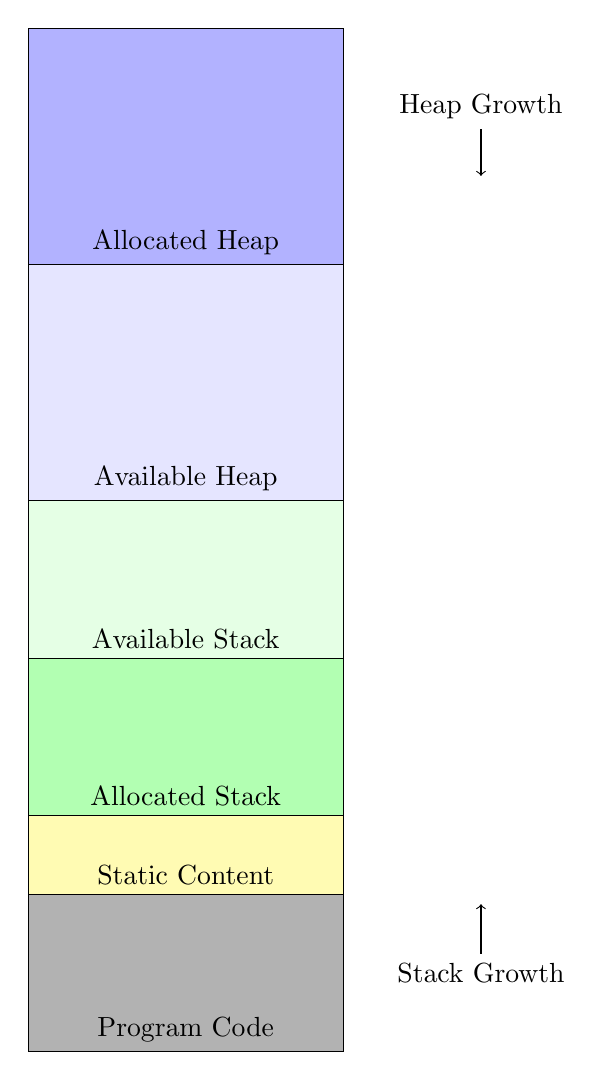
\begin{tikzpicture}[auto,scale=1.0,transform shape,every node/.style={text centered}]

%\path [top color=green!10!white, bottom color=white] (0,3) rectangle (6,5);

\path [draw,fill=black!30!white] (0,0) rectangle (4,2);
\path [draw,fill=yellow!30!white] (0,2) rectangle (4,3);
\path [draw,fill=green!30!white] (0,3) rectangle (4,5);
\path [draw,fill=green!10!white] (0,5) rectangle (4,7);
\path [draw,fill=blue!10!white] (0,7) rectangle (4,10);
\path [draw,fill=blue!30!white] (0,10) rectangle (4,13);

\node [above] (pc) at (2, 0) {Program Code};
\node [above] (static) at (2, 2) {Static Content};
\node [above] (ustack) at (2, 3) {Allocated Stack};
\node [above] (astack) at (2, 5) {Available Stack};
\node [above] (aheap) at (2, 7) {Available Heap};
\node [above] (uheap) at (2, 10) {Allocated Heap};

\node (sg) at (5.75, 1) {Stack Growth};
\node[above of=sg] (phantomsg) {~};
\draw[->] (sg) -- (phantomsg);

\node (hg) at (5.75, 12) {Heap Growth};
\node[below of=hg] (phantomhg) {~};
\draw[->] (hg) -- (phantomhg);

\end{tikzpicture}




\caption[Depiction of Application Memory.]{Depiction of Application Memory.  The details of
how application memory is allocated and how the stack/heap ``grow'' may vary depending
on the architecture.  The figure shows stack memory growing ``upward'' while heap allocation
grows ``downward.''  Allocation and deallocation may fragment the heap space though.}
\label{figure:stackAndHeap}
\end{figure}

Initially a program is allocated a certain amount of memory for its heap.
When a program attempts to dynamically allocate memory, say for a
new array of integers, it makes a request to the operating system for
a certain amount of memory (a certain number of bytes).  The system
responds by allocating a chunk of the heap memory which the program
can then use to store elements in the array.  Usually, the memory space
is stored as a pointer or reference.  The reference is stored in a variable
in a stack frame, but the actual contents of the array are stored in the
heap space.

Depending on the language and system, if a program uses all of its 
heap space and runs out, the operating system may terminate the program or it 
may attempt to reserve even more memory for the program.

\subsubsection{Memory Management}

If a program no longer needs a dynamically allocated memory space, 
it should ``clean up'' after itself by deallocating or ``freeing'' the memory, 
releasing it back to the heap space so that it can be reused either by 
the program or some other program or process on the system.
The process of allocating and deallocating memory is generally
referred to as \emph{memory management}.  If a program does not
free up memory, it may eventually run out and be forced to terminate.  
Even if it does not run out of available memory, its performance may 
degrade.  

If a program has poor memory management and fails to deallocate
memory when it is no longer needed, the memory ``leaks'': the available
memory is gradually lost because it is not released back to the 
heap for reallocation.  Programs which such poor memory management
are said to have a \gls{memory leak}\index{memory leak}. Sometimes
this is a consequence of a \gls{dangling pointer}: when a program
dynamically allocates a chunk of memory but then due to carelessness,
loses the reference to the memory chunk, making it impossible
to free up.

Some languages have automatic \gls{garbage collection} that
handle memory management for us.  The language itself is
able to monitor the dynamically allocated pieces of memory 
and determine if any variable in the program still references it.
If the memory is no longer referenced, it is ``garbage'' and
becomes eligible to be ``collected.''  The system itself then
frees the memory and makes it available to the program or
operating system.  In such ``memory managed'' languages, 
we are responsible for allocating memory, but are not (necessarily)
responsible for deallocating it.  

Even if a language offers automated memory management, 
it is still possible to have memory leaks and other memory
allocation issues.  That is, automated memory management
does not solve all of our memory management problems.  
Moreover, it comes at a cost.  The additional resources and
overhead required to monitor memory can have a significant
performance cost.  However, with modern garbage collection
systems and algorithms, the performance gap between
garbage collected languages and user-managed memory
languages has been shrinking.

In any case, all program memory is reclaimed by 
the operating system when the program terminates.

\section{Multidimensional Arrays}

A normal array is usually one dimensional.  One can think an array
as a single ``row'' in a table that contains a certain number of entries.
Most programming languages allow you to define \emph{multidimensional}
arrays.  For example, two dimensional arrays would model having
multiple rows in a full table.  You can also view two dimensional 
arrays as matrices in mathematics.  A \emph{matrix} is a rectangular
array of numbers that have a certain number of \emph{rows} and
a certain number of \emph{columns}.  

As an example, consider the following $2 \times 3$ matrix (it has
2 rows and 3 columns):
\[
\begin{bmatrix}
1 & 9 & -8 \\
2.5 & 3 & 5
\end{bmatrix}
\]
In mathematics, entries in a matrix are indexed via their row and column.
For example, $a_{i,j}$ would refer to the element in the $i$-th row and
$j$-th column.  Referring to the row first and column second is referred
to as \emph{row major} ordering.  If the number of rows and the number
of columns are the same, the matrix is referred to as a \emph{square matrix}.
For example, the following is a square, $10 \times 10$ matrix.
$$\left[ \begin{array}{cccccccccc}
 2 & 68 &  9 & 44 & 80 & 79 & 77 & 59 & 27 &  2 \\
 3 & 86 & 22 & 42 & 58 & 24 & 45 & 39 &  7 & 47 \\
 5 &  7 & 17 & 12 & 29 & 56 & 68 & 14 & 65 &  3 \\
 7 & 35 & 64 & 69 & 79 & 56 & 52 & 77 & 82 & 85 \\
11 & 55 & 36 &  5 & 25 &  6 & 22 & 25 & 72 & 37 \\
13 & 20 & 37 & 74 &  3 & 53 & 87 & 70 &  3 & 78 \\
17 & 72 & 68 & 26 & 11 &  6 & 63 & 70 & 29 & 16 \\
19 & 59 &  6 & 26 & 87 & 18 & 82 & 27 & 75 & 19 \\
23 & 73 & 30 & 80 & 51 & 14 & 34 & 67 & 59 & 58 \\
29 & 48 &  2 & 39 & 18 & 21 & 33 & 28 & 40 & 34 \\
\end{array} \right]$$

We can do something similar in most programming languages.  First,
languages may vary in how you can create multidimensional arrays, but
you usually have to provide a size for each dimension when you create 
them.  Once created, you can index them by providing multiple indices.
For example, with a two dimensional array, we could provide two indices
each in their own square brackets \mintinline{c}{arr[i][j]} referring to the
$i$-th row and $j$-th column.  Multidimensional arrays usually use the 
same 0-indexing scheme as single dimensional arrays.

You can further generalize this and create 3-dimensional arrays, 4-dimensional
arrays, etc.  However, the use cases for arrays of dimension 3 and
certainly for arrays of dimension $4$ or greater are rare.  If you 
need to store such data, it may be more appropriate to define a 
custom, user-defined structure or object (see Chapter \ref{chapter:objects})
instead of a higher dimensional array.

We usually think of 2-dimensional arrays as having the same number
of elements in each ``row''.  In the example above, both of the matrix's
rows had 3 elements in it.  Some languages allow you to create
2-dimensional arrays with a different number of elements in each
row.  Special care must be taken to ensure that you do not index an 
element that does not exist.

\section{Other Collections}

Aside from basic arrays, many languages have rich libraries of other
\emph{dynamic} collections.  Dynamic collections are not the same
thing as dynamically allocated arrays.  With a normal array, once 
created, its size is fixed and cannot, in general, be changed.  However,
dynamic collections can grow (and shrink) as needed when you 
add or remove elements from them.

\emph{Lists} are ordered collections that are essentially dynamic arrays.  
Lists are ordered and are usually zero-indexed just like arrays.  Lists
are generally objects and provide methods that can be used to add, 
remove, and retrieve elements from the list.  If you add an element
to a list, the list will automatically grow to accommodate it, so its size
is not fixed when created.  Two common implementations of lists are
array-based lists and linked lists.  Array-based lists use an array to
store elements.  When the array fills up, the list allocates a new, 
larger array to hold more elements, copying the original contents
over to the new array with a larger capacity.  Linked lists hold elements
in \emph{nodes} that are linked together.  Adding a new element
simply involves creating a new node and linking it to the last element
in the list.

Some languages also define what are called \emph{sets}.  Sets allow
you to store elements dynamically just like lists, but sets are generally
\emph{unordered}.  There is no concept of a first, second, or last 
element in a set.  Iterating over the elements in a set could result
in a different enumeration of the elements each time.  Elements in
sets are also usually unique.  For example, a set containing integers
would only ever contain one instance of each integer.  The value 10,
for example, would only ever appear once.  If you added 10 to a set
that already contained it, the operation would have no effect on the
set.

Another type of dynamic array are \emph{associative arrays} (sometimes
called \emph{dictionaries}).  An associative array
holds elements, but may not be restricted in how they are indexed.
In particular, a language that supports associative arrays may allow 
you to use integers or strings as indices, or even any arbitrary object.
Further, when using integers to index elements, indices need not
be fully defined nor contiguous.  In an associative array you could
define an element at index 5 and then place the next element at index
10, skipping index 6 through 9 which would remain undefined.

One way to look at associative arrays is as a \emph{map}.  A map
is a data structure that stores elements as key-value pairs.  Both 
they keys and values could be any arbitrary type (integers or strings)
or object depending on the language.  You could map account
numbers (stored as strings) to account objects, or vice versa.  Using
a smart data structure like a map can make data manipulation a
lot easier and more straightforward.





